\documentclass[12px]{article}
\usepackage[cjk]{kotex}
\usepackage[top=2cm, bottom=4.5cm, left=2.5cm, right=2.5cm]{geometry}
\usepackage{amsmath, amssymb}
\usepackage{enumerate}
\usepackage{graphicx}

\title{응용통계학 3장 연습문제 풀이}
\author{20181653 이강희}
\date{}

\begin{document}
\maketitle

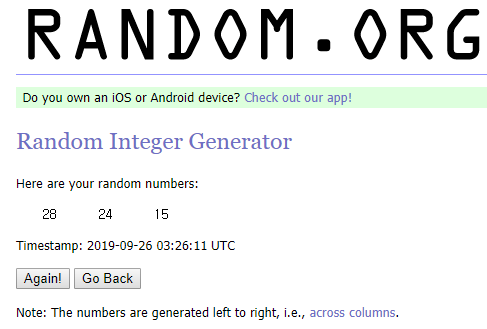
\includegraphics[scale=0.7]{random}

\section*{15번}
\begin{enumerate}[(1)]
    \item
    \(A \cup B \)의 확률은 \( P(A \cup B)= P(A) + P(B) - P(A \cap B) \) 이고,\\
    사건 A와 B가 서로 독립이기 때문에 \( P(A \cap B) = P(A) \times P(B) \) 이다.\\
    \begin{flalign*}
        P(A \cup B) &= P(A) + P(B) - P(A \cap B)&\\
        &=P(A) + P(B) - P(A) \times P(B)&\\
        &=0.3 + 0.6 - 0.3 \times 0.6&\\
        &=0.72&\\
    \end{flalign*}

    \item
    사건 B가 발생했을때 사건 A가 발생할 조건부확률은 \(P(A \mid B) = \frac{P(A \cap B)}{P(B)} \) 이고,\\
    사건 A와 B가 서로 배반이기 때문에 \(A \cap B = \varnothing, P(\varnothing) = 0 \) 이다.\\
    \begin{flalign*}
        P(A \mid B) &= \frac{P(A \cap B)}{P(B)}&\\
        &=\frac{0}{P(B)}&\\
        &=0&\\
    \end{flalign*}
\end{enumerate}

\section*{24번}
\begin{center}
    \begin{tabular}{ |c|c|c| } 
     \hline
     평가등급 & 재방문하겠다. & 재방문하지 않겠다. \\ 
     \hline
     상 & 0.40 & 0.05 \\ 
     중 & 0.20 & 0.10 \\ 
     하 & 0.05 & 0.20 \\
     \hline
\end{tabular}
\end{center}
\begin{enumerate}[(1)]
    \item
    표에서 재방문하겠다와 평가등급 상이 겹치는 부분은 0.40 이다.
    \item
    조건부 확률이다.\\
    전체 고객 중 재방문하겠다고 답한 고객의 비율은 \(0.40 + 0.20 + 0.05 = 0.65 \) 이고, 재방문하겠다고 답한 고객 중 평가등급 상이라고 답한 고객의 비율은 0.40이다.\\
    따라서 \(\frac{0.40}{0.65} = \frac{8}{13} \) 이다.
    \item
    이것도 조건부 확률이다.\\
    전체 고객 중 평가등급 상으로 답한 고객의 비율은 \(0.40 + 0.05 = 0.45 \) 이고, 평가등급 상으로 답한 고객 중 재방문할 것이라고 답한 고객의 비율은 0.40 이다.\\
    따라서 \(\frac{0.40}{0.45} = \frac{8}{9} \) 이다.
\end{enumerate}

\section*{28번}
선수 중 왼손잡이의 비율이 35\% 이므로\\
임의로 한 선수를 선택했을 때 그 선수가 왼손잡이일 확률을 \(P(A) = 0.35 \) 라 한다.\\
오른손잡이일 확률은 \(P(A^C) = 0.65 \) 이다. (양손잡이는 고려하지 않음)
\begin{enumerate}[(1)]
    \item
    두 선수 모두 왼손잡이일 확률은 \(P(A) \times P(A) =  0.1225 \) 이다.
    \item
    한 선수는 왼손잡이, 한 선수는 오른손잡이일 확률은\\
    \(P(A) \times P(A^C) = 0.35 \times 0.65 = 0.2275 \) 이다.
    \item
    적어도 한 선수는 오른손잡이일 확률은 모두 왼손잡이일 확률의 여집합이므로\\
    \(1 - P(A) \times P(A) = 1 - 0.1225 = 0.8775 \) 이다.
\end{enumerate}

\end{document}